\documentclass{article} % For LaTeX2e
\usepackage{nips15submit_e}
\usepackage{hyperref}
\usepackage{url}
\usepackage{float}
\usepackage{graphicx}
\usepackage{caption}
\usepackage{subcaption}
\usepackage{capt-of}
%\documentstyle[nips14submit_09,times,art10]{article} % For LaTeX 2.09


\title{Making Music with Hidden Markov Models}


\author{
Anna Yanchenko \\
Duke University\\
\texttt{anna.yachenko@duke.edu} \\
\And
Megan Robertson \\
Duke University \\
\texttt{megan.robertson@duke.edu} \\
}


\newcommand{\fix}{\marginpar{FIX}}
\newcommand{\new}{\marginpar{NEW}}

\nipsfinalcopy % Uncomment for camera-ready version

\begin{document}


\maketitle

\begin{abstract}
We use Hidden Markov Models (HMM) to capture the latent elements involved in music creation. The observed states are the notes and velocity, volumes, of each note. The latent states include elements such as chord progression, dynamics and patterns.In this paper, we implement three different Hidden Markov Models and compare the resulting compositions for each model. These models are trained on various classical piano pieces, and the resulting compositions are compared.
\end{abstract}
 
\section{Introduction}

Hidden Markov Models are known for their use in language applications such as speech recognition and handwriting recognition programs. However, it is also possible to use Hidden Markov Models in another language application, the language of music. This project serves as a platform to combine our shared interests of music and statistics. 

The project uses music data in the form of  Musical Instrument Digital Interface (MIDI) files. This interface creates a form of communication between computers and musical instruments that enables them to send instructions back and forth. MIDI files can contain multiple channels that store information about the notes and velocity of certain instruments. The files also contain information about when a particular note starts and stops. \footnote{MIDI Manufacturers Association, "An Introduction to MIDI"}. 

Any musician or student of music can tell you that there is more to composing music beyond stringing together some notes with a catchy rhtyhm. There are many things to consider such as chord progression, dynamics, and patterns. It is importnat for a composer to be fmant for a composer to be familar with things such as the Circle of Fifths. There are also different forms, sonata, rondo, blues and more, that can be used in the creation of music.\footnote{Music Composition for Dummies, \url{http://www.dummies.com/how-to/content/music-composition-for-dummies-cheat-sheet.html}}

However, the MIDI data does not capture all of the theory and ideas that create a composition. Therefore, we use Hidden Markov Models (HMMs) in order to capture both the observed states, the note/velocity information, as well as the latent variables, theory such as that described above. We utitilze three different HMMs and train them on classical piano pieces. The estimated parameters are then used to compose new pieces.


\section{Methods}

Classical piano pieces were used to train each of the models. In this paper we present the result forGustav Holt's Jupiter from "The Planets" and Johann Pachelbel's Canon. A piano arrangement of Jupiter was used as opposed to the orchestral piece. The MIDI files for these songs were converted to Comma Separated Value (CSV) files.\footnote{This was done using a program found at \url{http://www.fourmilab.ch/webtools/midicsv/}} 

The classical pieces were used to estimate the respective parameters of the models described below. In this training, the tempo, key signature and length of the original song were not changed. The only possible observed states were the velocities and notes present in the original pieces. Once the parameters had been estimated, they were used to generate a new piece of music. This process generates a CSV file of the new composition, and this file is then converted to a MIDI file using the same program as above. The files can then be played on a synsthesizer or a program such as GarageBand.

The three models used are described in the subsections below. They are a first order HMM, a second order HMM, and a first order HMM with two hidden states. 

- Transition matrix is the only thing changing between these models

\subsection {Model 1: First Order Hidden Markov Model}

The simplest of the three models is the first order Hidden Markov Model. In this model, the observed values, $X_i$, are the notes and their velocity. The model has only one hidden state for each note/velocity pair, $Z_i$, and each hidden state only depends on the prior hidden state. 

\begin{figure}[H]
\centering
\caption{Graphical Model - First Order HMM}
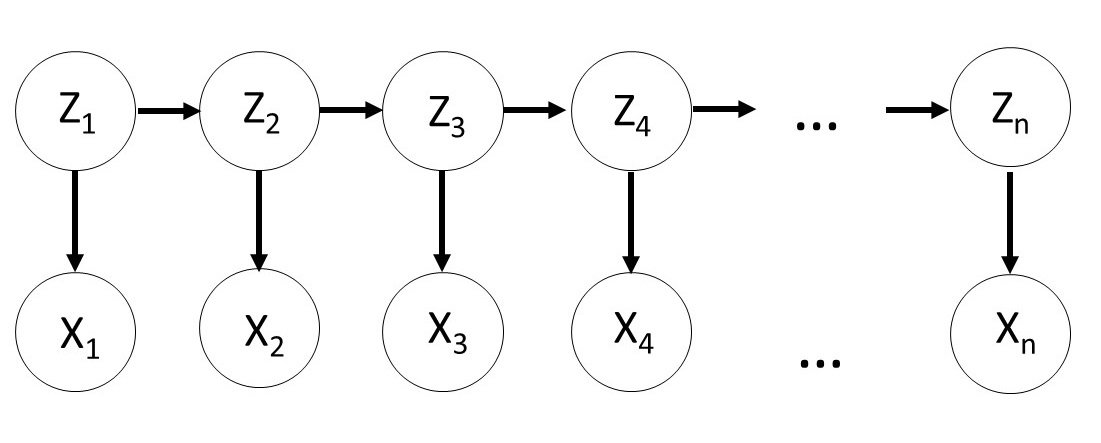
\includegraphics [scale = 0.35] {Model1.jpg}
\end{figure}

The Baum-Welch Alogirithm was used to estimate the parameters of this model. For details of the derivations and algorithm see class notes. \footnote{Statistics 531, Duke University Spring 2016. Instructor: Jeff Miller}
 
\subsection{Model 2: Second Order Hidden Markov Model}

The second model expanded on Model 1 by assuming that each state also depended on the prior two states. This enables the model to capture the structure that is evolving over time in the piece. The Baum-Welch Algorithm was again used to estimate the parameters. The details of the algorithm for this model can be found in Mari and Schott's "Probabilistic and Statsitical Methods in Computer Science." \footnote{Jean-Francoix Mari and Rene Schott, "Probabilistic and Statistical Methods in Computer Science", Springer Science, pg. 161-167 and Brett Watson and Ah Chung Tsoi, "Second Order Hidden Markov Models for Speech Recognition", Univsersity of Queensland}.

\begin{figure}[H]
\centering
\caption{Graphical Model - Second Order HMM}
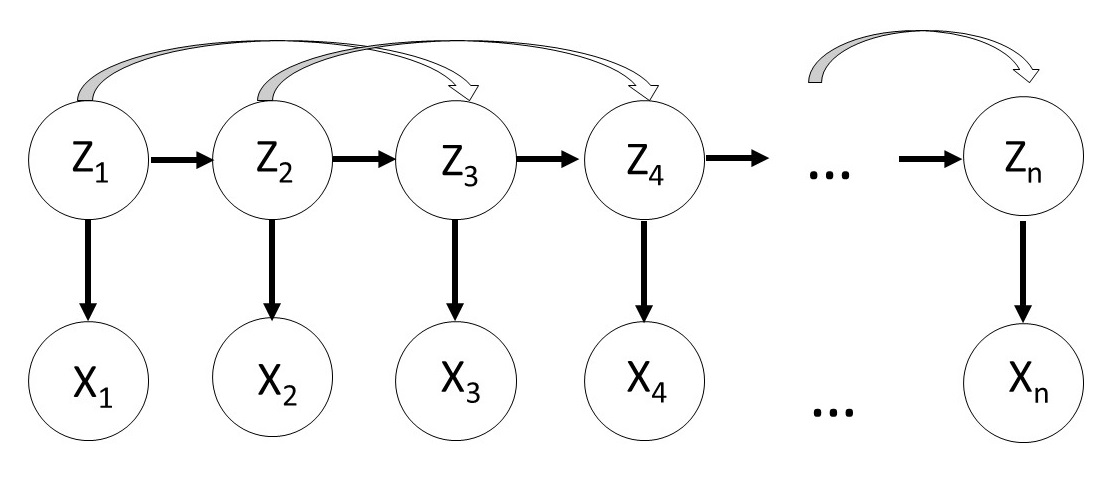
\includegraphics [scale = 0.35] {Model2.jpg}
\end{figure}

\subsection{Model 3: HMM with Two Hidden States}

The final model expanded on the intital model by adding a second latent variable. This meta-state allows the model to capture additional aspects of the hidden states and the music generation process.  This processes might evolve at a rate different than the processes that are present in the observed states and one latent state. 

\begin{figure}[H]
\centering
\caption{Graphical Model - First Order HMM with Two Hidden States}
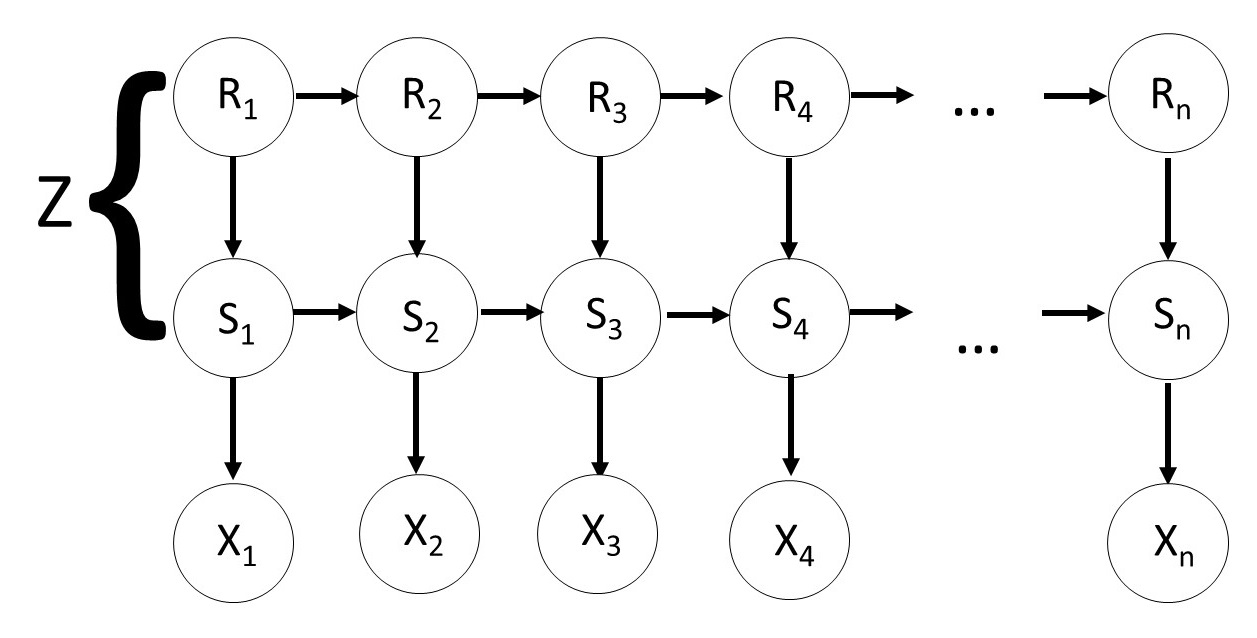
\includegraphics [scale = 0.35] {Model3.jpg}
\end{figure}

For the derivation of the Baum-Welch algorithm for this model, see the Appendix.

\section{Results}

\subsection{Original Pieces}

Of the four pieces used to train the various models, Jupiter and Pachabel's Cannon provided the best results. It is possible that these pieces performed the best because of their prominent melody from the beginning. For example, in Claude Debussy's Clair de Lune, the piece builds for a while before the melody emerges. Our models may not have worked well for this because they did not have the capability to capture the building structure and melody of the song. 

\begin{figure}[H]
\centering
\caption{Jupiter - Original Song}
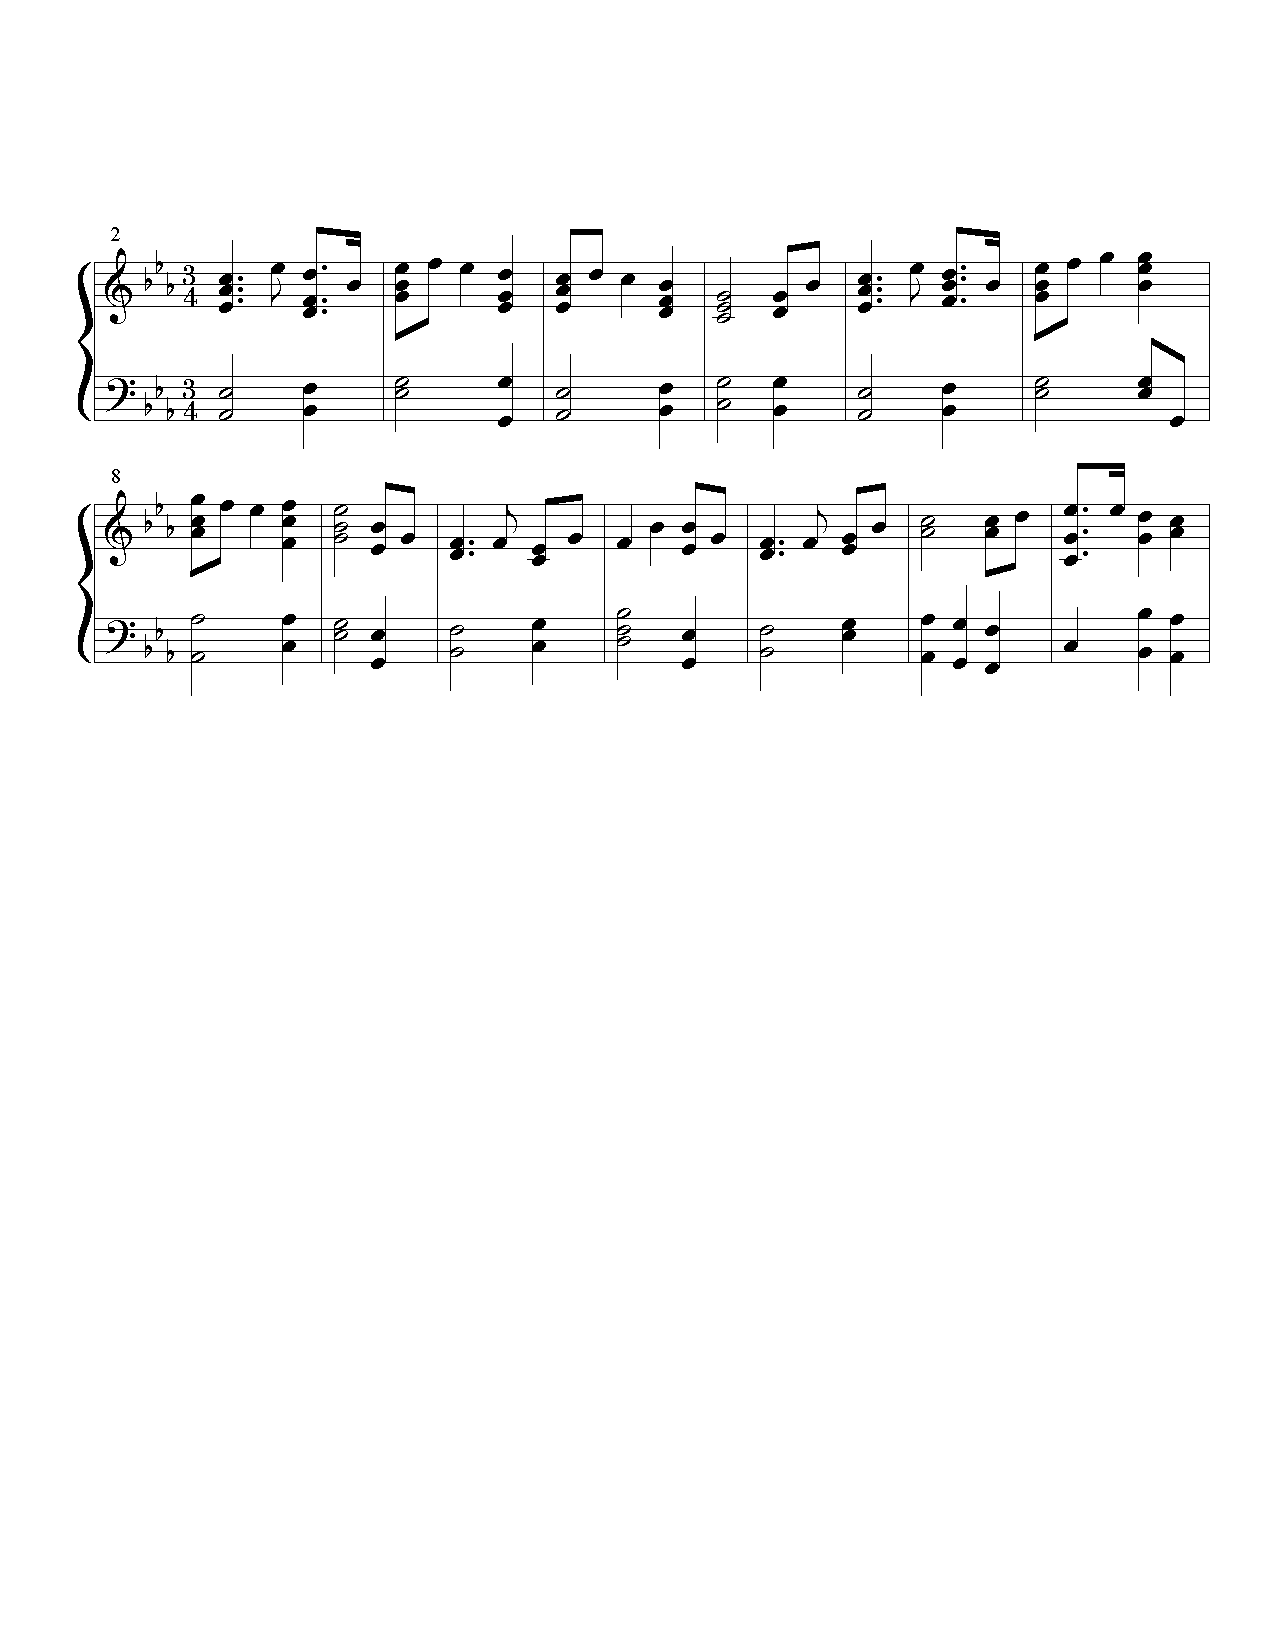
\includegraphics [scale = 0.6] {JupiterOriginal-cropped.pdf}
\end{figure}

Both Jupiter and Pachabel's Cannon are well-known classical pieces whose themes occur frequently in advertisements and other media forms. The two pieces have a logical progression. It is obvious that these pieces are structurally sound and musically cohesive given their notoriety. 

\subsection{First Order Hidden Markov Model}

-lots of octave interval jumps that are not apparent in the actual song (measures 1, 3, 4 and more)
- more rests in the first two lines
- more quarter and half notes than in the original piece (for the right hand - top)
- left hand moves more than originally and the left hand has less moving notes, melody seems to be equally distributed between the two hands
- also no resolution

\begin{figure}[H]
\centering
\caption{Jupiter Remix - Model 1}
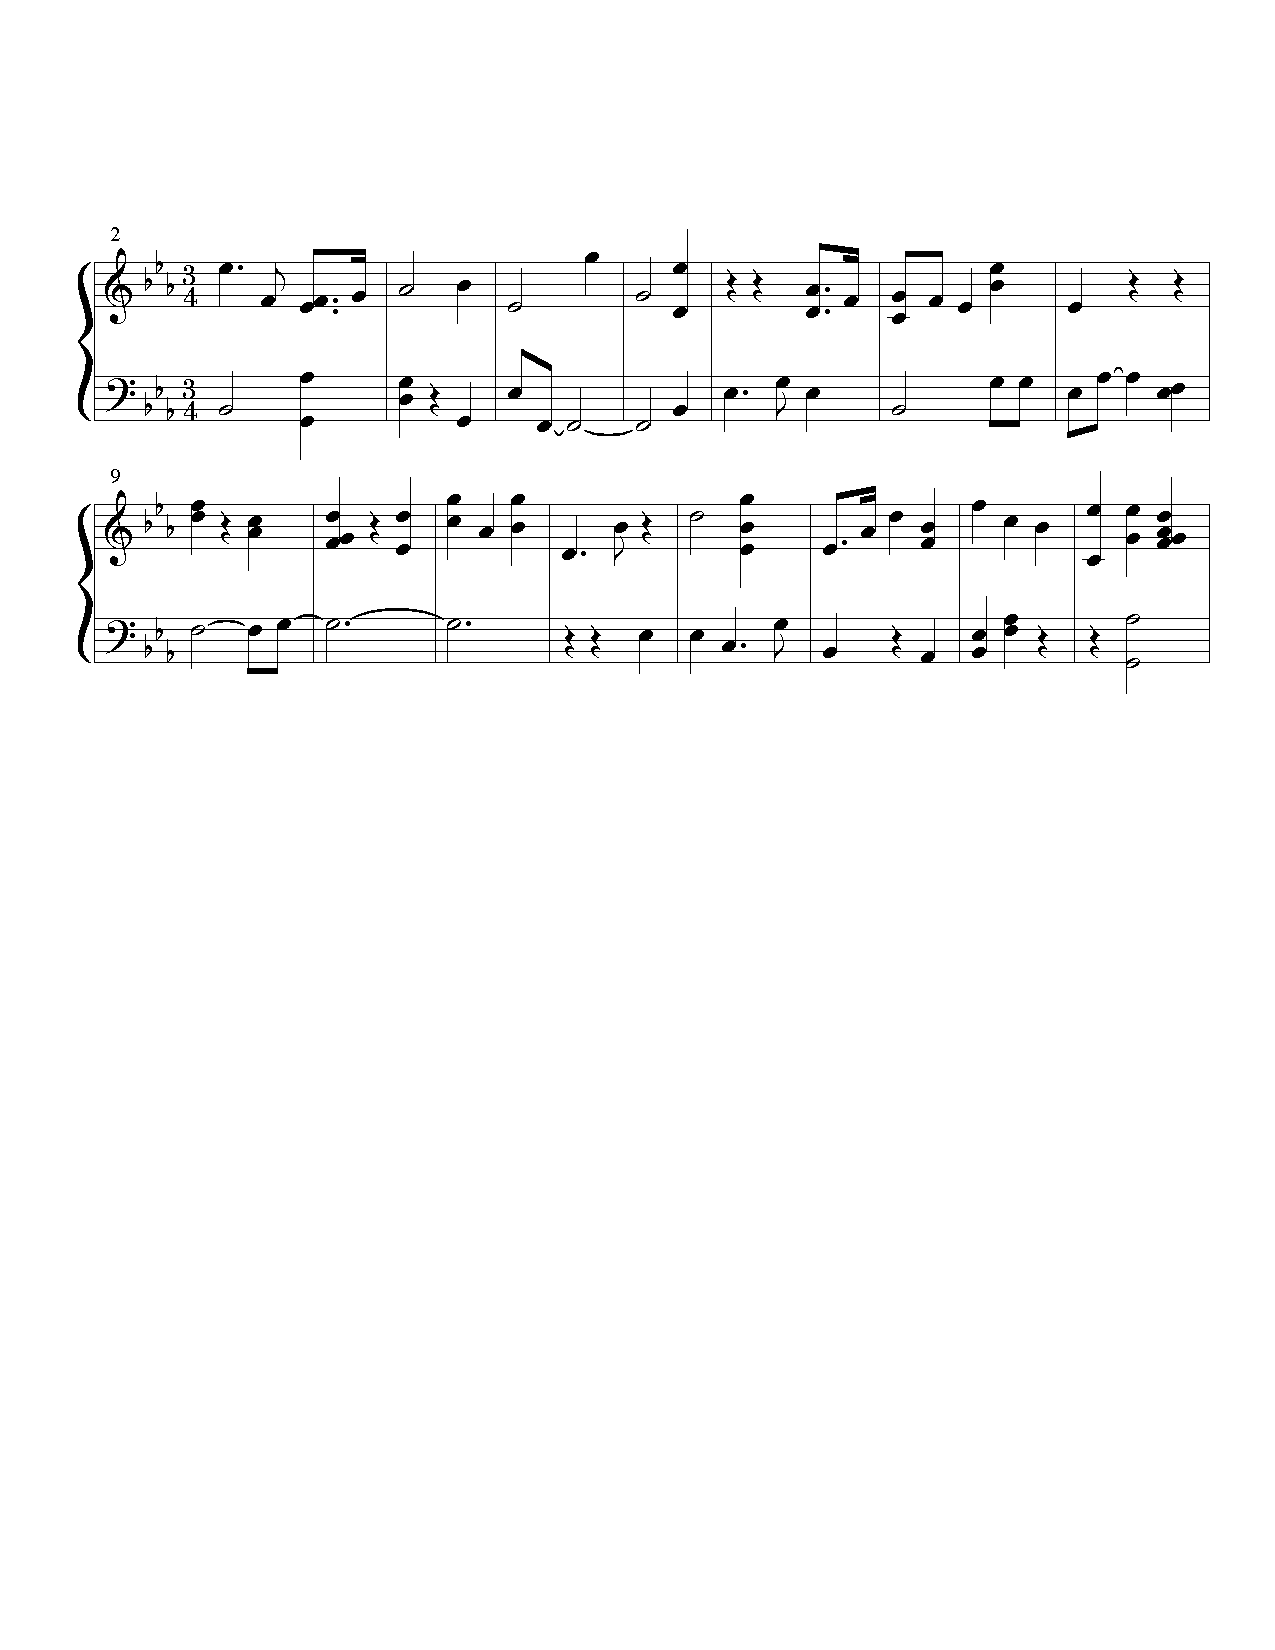
\includegraphics [scale = 0.6] {JupiterRemix-cropped.pdf}
\end{figure}

Pachabel's
-fewer sixteenth notes and more dotted notes (beat and a half)
- original has mostly all straight eighth/sixteenth notes for the melody
- more rests than there are in the original 
- large octave jumps that don't occur, also just some large intervals


Why do we think this is happening
- melody for Pachabel's builds over several measures, only basing on previous note
- not capturing enough of overall structure, so some notes are occuring together that should not occur together
- more structure would get whole chord from the prevous state, so some notes are dissonant together

Survey results

\subsection{Second Order Hidden Markov Model}

Jupiter
-still some large interval jumps, but less than model one
-chords make more sense but there is less dissonance
-less rests than model one but more than in the original


SURVEY SAYS


\begin{figure}[H]
\centering
\caption{Jupiter Remix - Model 2}
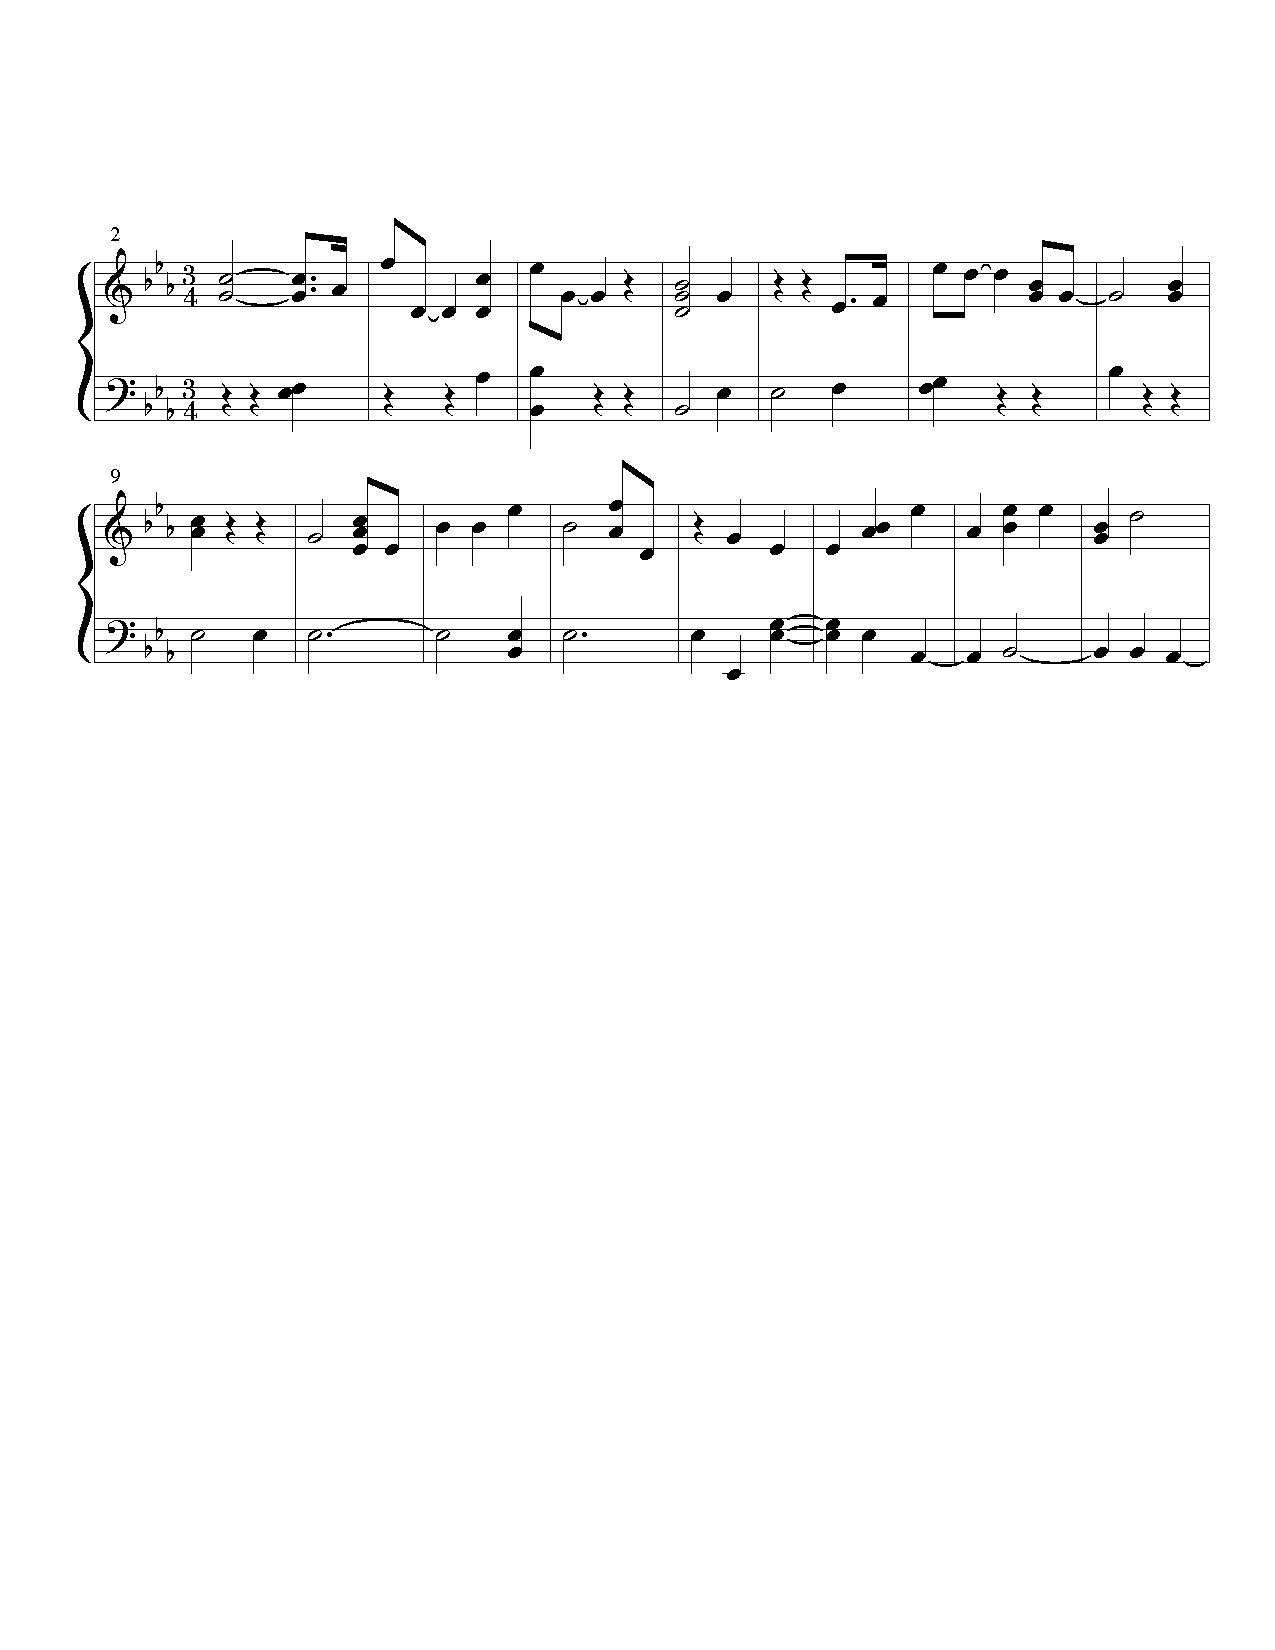
\includegraphics [scale = 0.6] {JupiterRemix2-cropped.pdf}
\end{figure}

Pachabel
-more sixteenth notes than the first order but less than the original song
-awkward interval jumps present
-chords made more sense, less dissonance, gaps and breaks


-progression of the song seemed more logical because more structure was being captured than the original version


\subsection{First Order Hidden Markov Model with Two Hidden States}

Jupiter 
- fewest rests of the three remixes, but stil more than the original
-interval jumps are larger than original, but smaller than the other songs and there are fewer of them


\begin{figure}[H]
\centering
\caption{Jupiter Remix - Model 2}
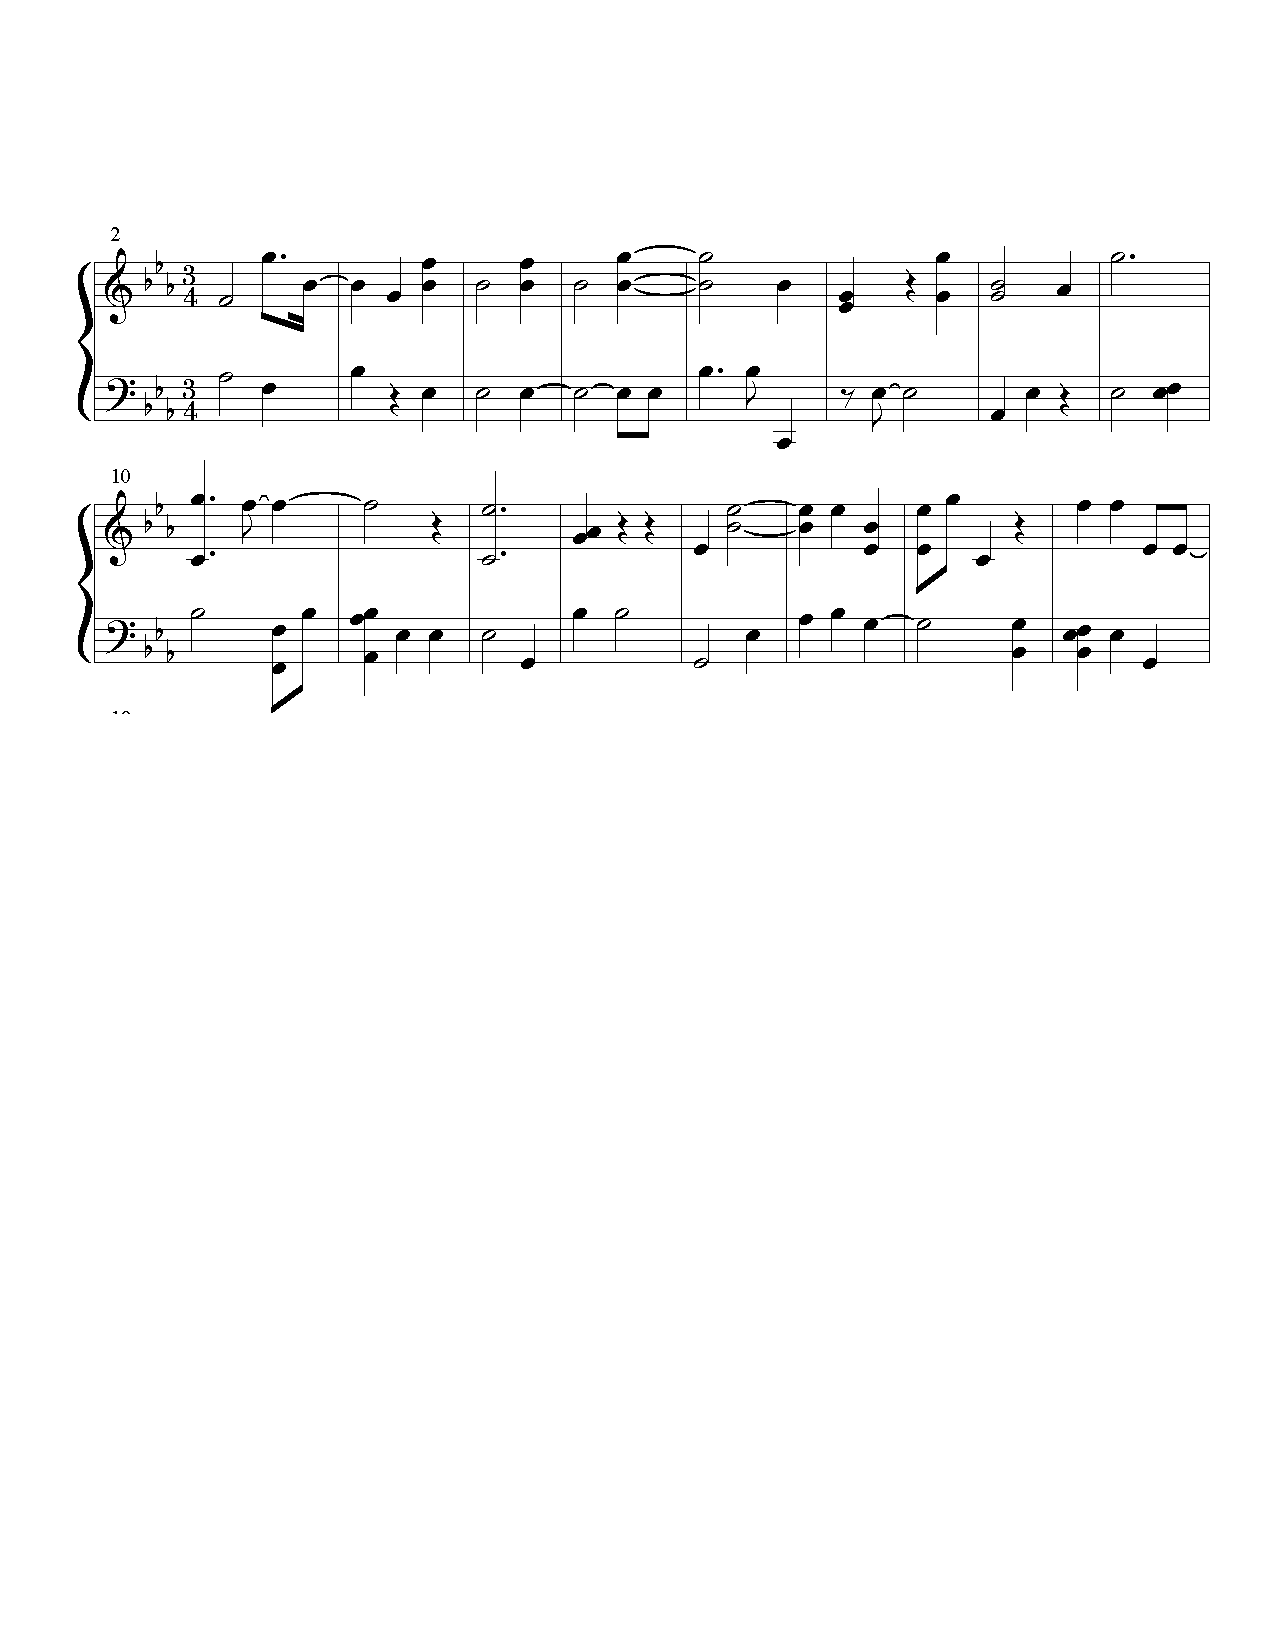
\includegraphics [scale = 0.6] {JupiterRemix2H-cropped.pdf}
\end{figure}

*Pachabel*
-lots of eighth and sixteenth notes, more than the other two but not as many as the original
-still large jumps in notes, eight or more, between successive notes (including half steps) (see this measure for an example)

\subsection{Summary}
- Model 2 appears to be better with structure
- Model 3 has better chords
- in all of the models, the melody seemed to be split between the two hands, models did not catch that in general the lower notes were longer and most of the melody was in the right hand notes
- dynamics modeled independently, so didn't always line up logically

\section{Conclusion and Further Research}

Conclusion 
-none of our models fully capture music, DUH
- at certain points, there are some measures that are good, but not capturing enough structure for the overall piece to be cohesive
- need to connect all of these little victories
-second state seemed to work best 

-consider higher state models, perhaps 3-5 (adding the second hidden state got considerably better musically)
- determine how to use for a multiple instrument piece
- model dependendcies between dynamics and the notes, not treat them as indpendent

-incorporating these changes could improve the musicality of our remixes


\newpage

\section{Appendix}

\subsection{Baum-Welch for First Order HMM with Two Hidden States}

Define the following:

$$A_{ij} = \textbf{P} (R_t = j | R_{t-1} = i)$$
$$B_{jkl} = \textbf{P} (S_t = l | R_t = j, S_{t-1} = k)$$ 
$$T_{ik, jl} = A_{ij} B_{jkl} = \textbf{P} (R_j = j, S_t = l | R_{t-1} = i, S_{t-1} = k)$$
$$Z_t = (R_t, S_t)$$

The constraints are $\sum_j A_{ij} = 1, \sum_l B_{jkl} = 1.$ \newline

Define c to be a constant. Thus,  \newline
$$Q(\theta, \theta_k) = c + \sum_{t=2}^n \sum_{i,k} \sum_{j,l} \textbf{P}_{\theta_k} (R_{t-1} = i, S_{t-1} = k, R_t = j, S_t = l | x) log T_{ik, jl}$$ 
$$B_{tikjl} = \textbf{P}_{\theta_k} (R_{t-1} = i, S_{t-1} = k, R_t = j, S_t = l | x)$$
$$log T_{ik, jl} = log A_{ij} + log B_{jkl}$$

Thus, \newline
$$ 0 = \frac{\partial}{\partial A_ij}(Q(\theta, \theta_k) - \lambda \sum_{j} A_{ij}) = (\sum_{t=2}^n \sum_k \sum_l B_{tiklj} \frac{1}{A_{ij}}) - \lambda$$
$$\lambda A_{ij} = \sum_{t=2}^n \sum_k \sum_l B_{tikjl}$$
$$\lambda = \sum_j \sum_{t=2}^n \sum_k \sum_l B_{tiklj}$$

For each i, $A_{ij} \propto \sum_{t=2}^n \sum_{k,l} B_{tikjl}$ \newline

$$ 0 = \frac{\partial}{\partial B_{jkl}} (Q(\theta, \theta_k) - \lambda \sum_l B_{jkl}) = \sum_{t=2}^n \sum_i B_{tiklj} \frac{1}{B_{jkl}} - \lambda$$
$$ \lambda B_{jkl} = \sum_{t=2}^n \sum_i B_{tikjl}$$

For each j, k, \newline
$$B_{jkl} \propto \sum_{t=2}^n \sum_i B_{tikjl}$$

\newpage

\section{References}
\begin{enumerate}
\item Wattson, Brett and Ah Chung Tsoi. "Second Order Hidden Markov Models for Speech Recognition", University of Queensland, 146-151. 
\item MIDI Manufacturers Association, "An Introduction to Midi". 
\item Music Composition for Dummies, http://www.dummies.com/how-to/content/music-composition-for-dummies-cheat-sheet.html
\end{enumerate}

\end{document}